
\section{Verbesserter Algorithmus von Wetherell und Shannon}
\label{chap:kapitel3_2}
\erstelltvon{Treulieb}
Wetherell und Shannon stellen in Ihrem Paper einen weiteren, verbesserten Algorithmus zum Zeichnen von Bäumen vor, welcher jedoch
ausschließlich Binärbäume zeichnen kann. Dieser Algorithmus weist die Nachteile des naiven Algorithmus nicht mehr auf.
Dafür definieren sie zwei weitere Anforderungen, die der Algorithmus erfüllen soll. Jene Anforderungen sind speziell für Binärbäume.   

\begin{quotation}
	\textit{Aesthetic 2:} In a binary tree, each left son should be positioned
	left of its father and each right son right of its father\cite[]{q1}.
\end{quotation}

In einem Binärbaum hat jeder Knoten maximal ein linkes und maximal ein rechtes Kind. Daher ist es auch logisch, dass jedes linke Kind 
links vom Vater und jedes rechte Kind rechts vom Vater positioniert werden soll. Zudem soll jeder Vater zentriert über seinen Kindern
stehen. Dieses Verhalten legen Wetherell und Shannon in einer weiteren Anforderung fest.

\begin{quotation}
	\textit{Aesthetic 3:} A parent should be centered over its children\cite[]{q1}.
\end{quotation}

Im Folgenden wird direkt die modifizierte Version des verbesserten Algorithmus betrachtet. Dafür wird die zweite While-Schleife des Programmcodes
mit der Fig. 9 \cite[A modification of Algorithm 3]{q1} ersetzt.

\label{chap:kapitel3_2_Ablauf}
\subsection{Ablauf}
\erstelltvon{Garan}

Dieser Algorithmus lässt sich in zwei Phasen unterteilen. In der ersten Phase wird die vorläufige X-Koordinate der einzelnen Knoten bestimmt.
In der zweiten Phase werden diese X-Koordinaten bei Bedarf nochmals abgeändert sowie die Y-Koordinate berechnet.

Dieser Algorithmus besitzt zwei Eingabeparameter, nämlich die Wurzel des Baumes und die Höhe des Baumes. Zu Beginn werden zwei
ganzzahlige Arrays, ein Positions-Array und ein Modifikator-Array, definiert. Diese besitzen die Länge "Höhe des Baumes".
Hiernach müssen alle Elemente des Positions-Array mit eins und alle Elemente des Modifikator-Array mit null initialisiert werden.
Zudem wird eine Variable namens "ModifikatorSumme" deklariert und mit null initialisiert.

Nun wird über die Baumstruktur in der Post-Order traversiert. Dabei werden die vorläufigen X-Koordinaten der Knoten wie folgt bestimmt:
Bei der Bestimmung der X-Koordinate wird zwischen vier verschiedenen Fällen unterschieden:
\begin{enumerate}
	\item Der Knoten ist ein Blatt (er besitzt weder ein linken noch rechtes Kind)
	\item Der Knoten besitzt kein linkes Kind
	\item Der Knoten besitzt kein rechtes Kind
	\item Der Knoten besitzt zwei Kinder (links und rechts)
\end{enumerate}

Im ersten Fall entspricht die X-Koordinate dem Eintrag im Positions-Array in Abhängigkeit zu seiner Höhe.
Im zweiten Fall wird der Knoten links, mit einem Offset von eins, von seinem rechten Kind positioniert.
Im dritten Fall wird dieser rechts, mit einem Offset von eins, von seinem linken Sohn positioniert. Im letzten Fall wird der Knoten
in der Mitte zwischen seinen Kinder positioniert. Hierbei kann die folgende Formel genutzt werden: $$x = (left.x + right.x) / 2.$$
Hiernach wird der Modifikator bestimmt. Dafür wird der der größere Wert des entweder bereits existierenden Modifikator der Ebene genommen
oder wie folgt berechnet: die nächste freie Position der Ebene subtrahiert mit der zuvor berechneten X-Koordinate.
Nun wird der Wert im Position-Array am Index (Höhe des Knotens im Baum) wie folgt neu berechnet:
X-Koordinate des Knoten plus eins. Zusätzlich wird der spezifische Modifikator des Knotens gesetzt
(Wert aus dem Modifikator-Array am Index: Höhe des Knotens im Baum).

In der zweiten Phase wird zu Beginn eine Variable namens "ModifikatorSumme" deklariert und mit null initialisiert.
Hiernach wird über die Baumstruktur in einer modifizierten Pre-Order traversiert. Die ModifikatorSumme entspricht
der Summe aus allen Modifikatoren der Väter eines Knotens. Um diese Summe zu berechnen wird bei dem Besuch eines Kind-Knotens
der spezifische Modifikator des Vaters auf die Summe addiert. Beim Übergang eines Kindes zurück auf den Vater wird entsprechend
der knotenspezifische Modifikator von der globalen ModifikatorSumme abgezogen.

Da die Pre-Order Traversierung vorgibt, erst den linken Teilbaum, dann den Knoten und zum Schluss den rechten Teilbaum zu besuchen,
wird zunächst beginnend von der Wurzel aus, der am weitesten links unten stehende Knoten besucht. Abbildung \ref{pic:baum_algo_2}
zeigt einen Baum, welcher mit dem verbesserten Algorithmus gezeichnet wurde. In diesem Beispiel wird bei der Wurzel gestartet 
und nach Knoten D gelaufen. Auf dem Weg dorthin werden die Modifikatoren von A und B auf die globale ModifikatorSumme addiert.
Danach wird die X-Koordinate des Knotens entweder auf die nächste freie X-Koordinate auf der Höhe des Knotens gesetzt oder auf den
Wert der vorläufigen X-Koordinate addiert mit der ModifikatorSumme. Dabei wird der kleinere der beiden Werte genutzt, um sicherzustellen,
dass der Knoten möglichst weit links ist. Wenn der Knoten einen linken Sohn hat und die X-Koordinate des Sohnes größer ist als
die X-Koordinate des Vaters, dann wird die X-Koordinate des Vaters auf die X-Koordinate des Sohnes plus eins gesetzt. 
Damit wird sichergestellt, dass der Knoten nicht direkt über seinem linken Sohn steht, sondern eine Position weiter rechts.
Falls der Knoten nicht die Wurzel ist, der Vater des Knotens bereits besucht und abgearbeitet wurde und die X-Koordinate des Knotens
kleiner als die X-Koordinate des Vaters plus eins ist, dann wird die X-Koordinate des Knotens auf die X-Koordinate des Vaters plus eins gesetzt.
Ähnlich wie im Fall vorher dient diese Überprüfung dazu, den Knoten richtig zu positionieren. Hier wird dadurch verhindert,
dass der Knoten genau unter seinem Vater steht. Stattdessen wird sichergestellt, dass der Knoten rechts von seinem Vater steht,
welcher der rechte Sohn sein muss, da der Vater bereits besucht und positioniert wurde. Nun ist die X-Koordinate des Knotens final
bestimmt worden. Die Y-Koordinate wird genau wie im naiven Algorithmus bestimmt, indem die Höhe des Knotens mit zwei multipliziert
und mit einem Offset (hier eins) addiert wird. Zum Schluss wird die nächste freie X-Position auf der Höhe des Knotens bestimmt,
indem die X-Koordinate mit einem Offset (hier zwei) addiert wird. 


\subsection{Implementierung in Java}
\erstelltvon{Treulieb}

\begin{figure}[H]
    \centering
    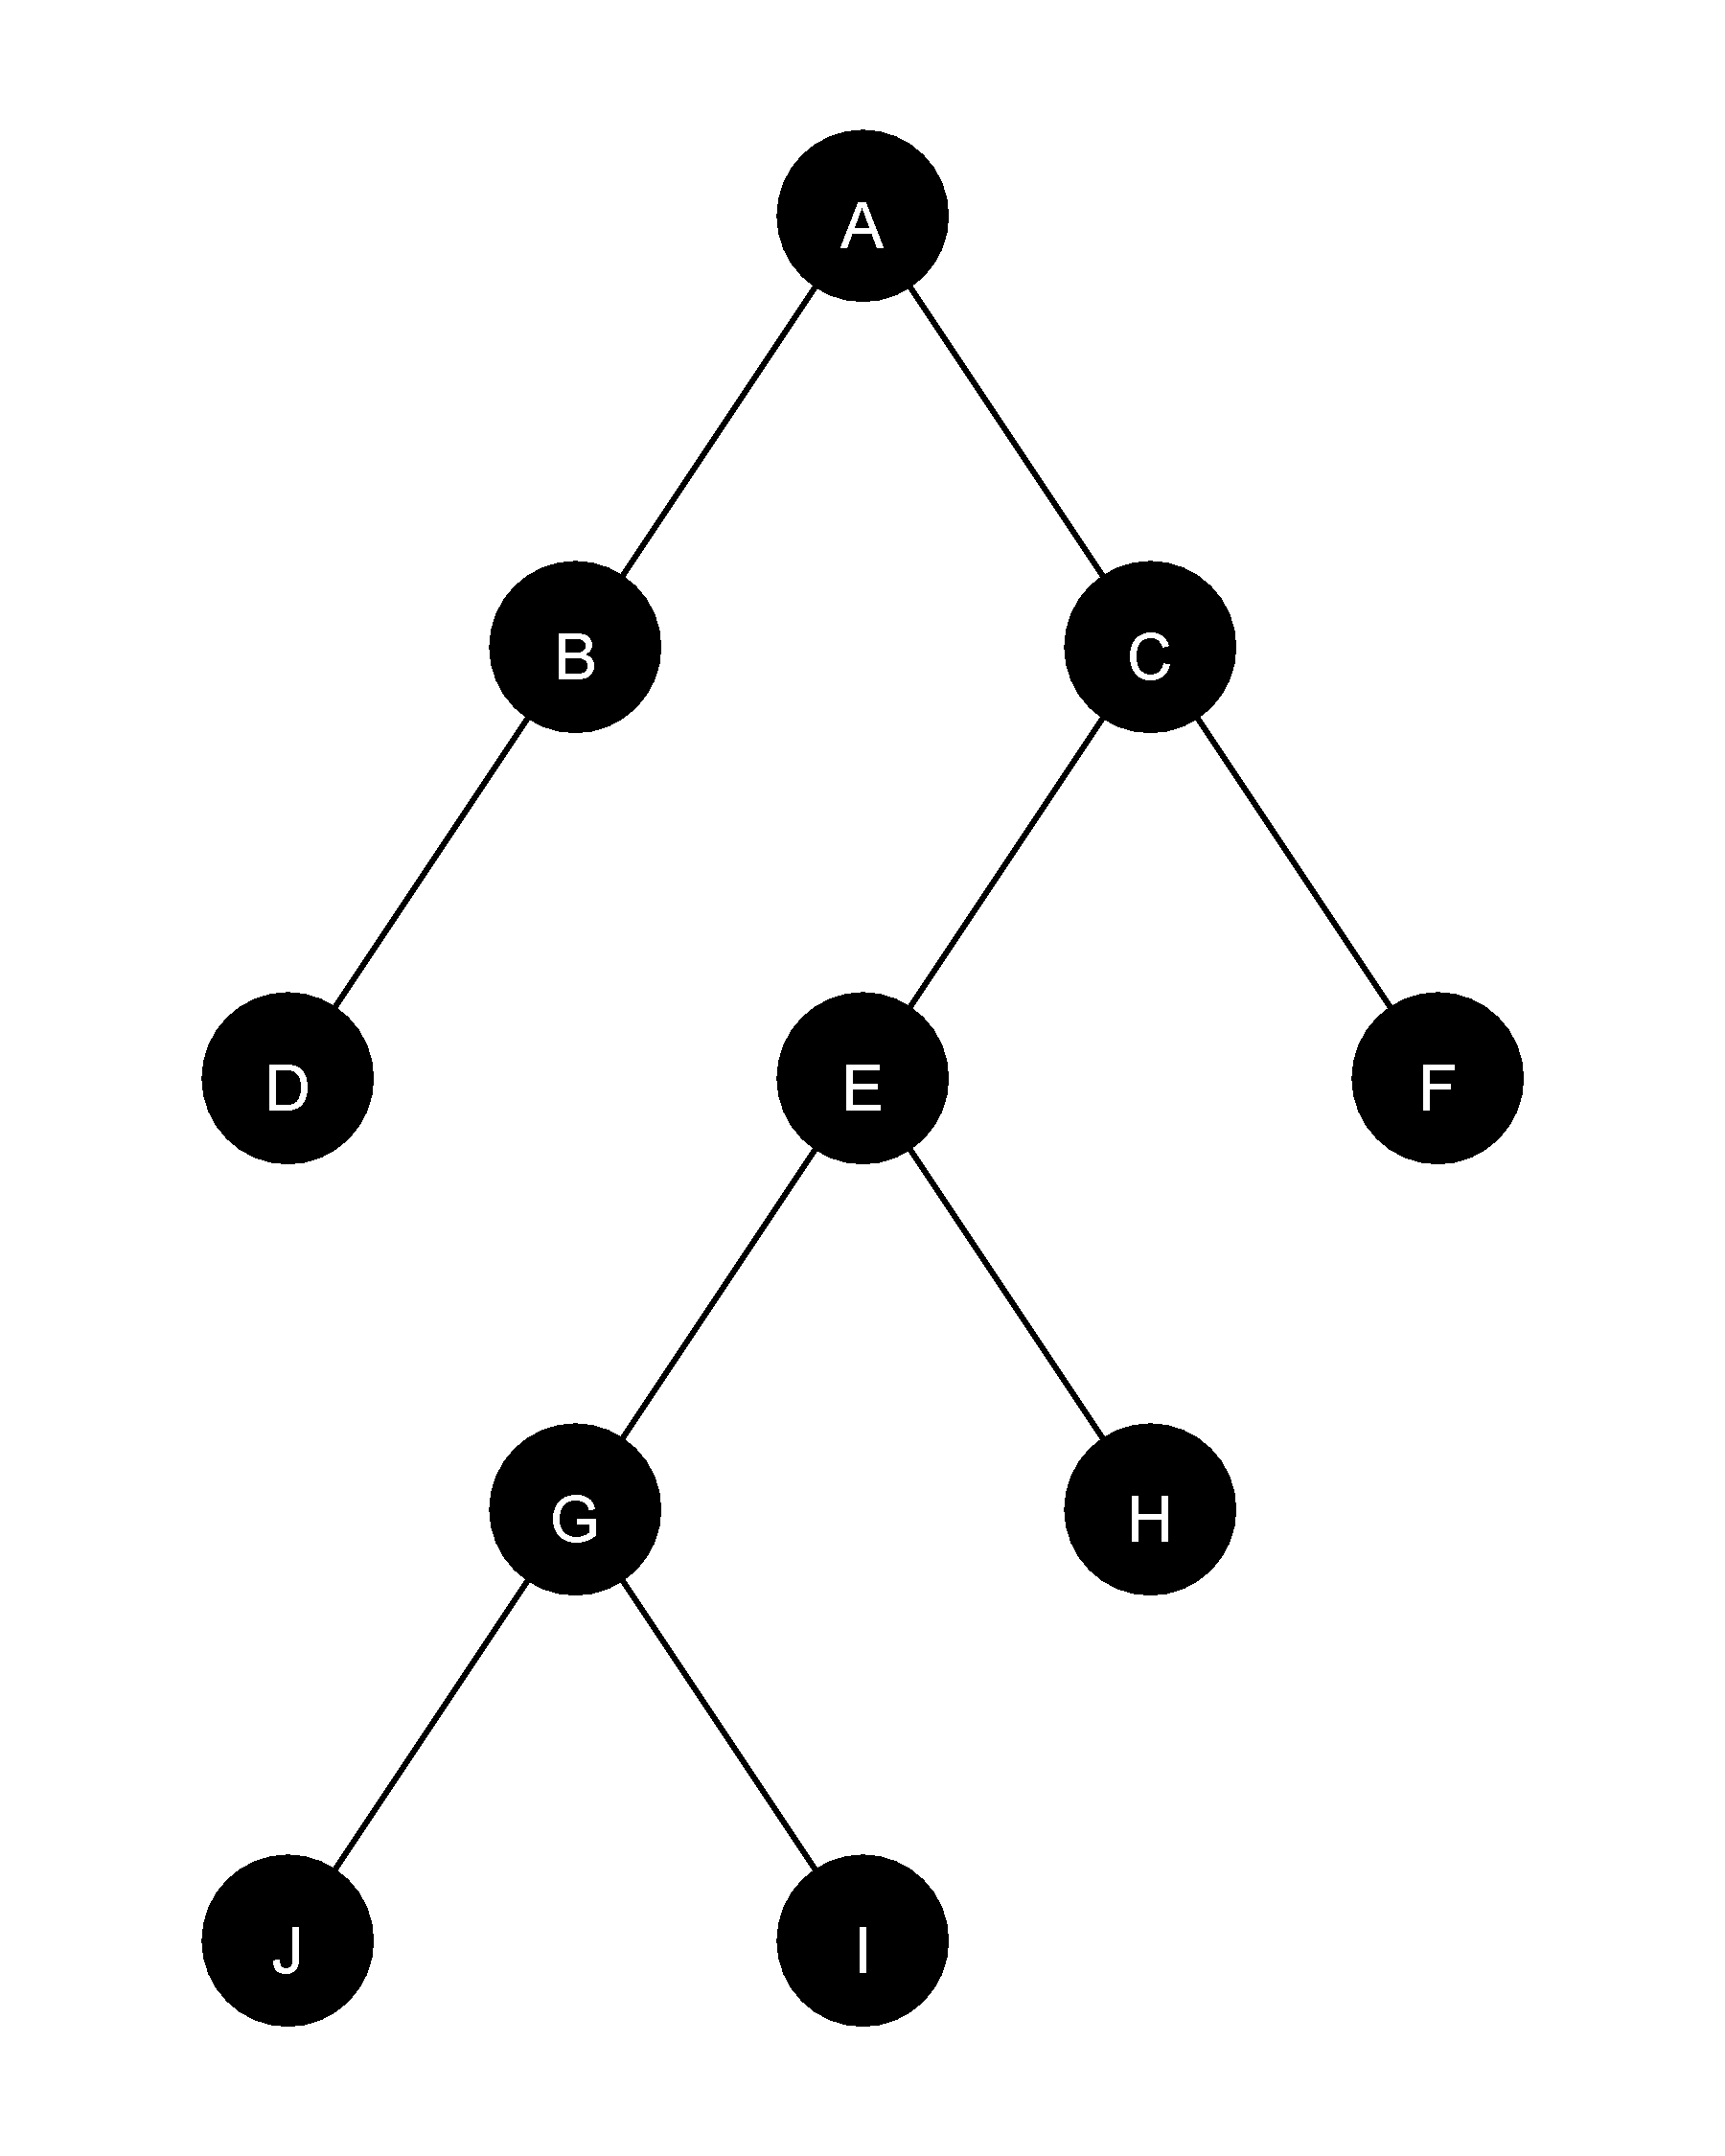
\includegraphics[scale = 0.10]{abbildungen/baum_algo_2}
    \caption{Gezeichneter Baum durch den verbesserten Algorithmus}
    \label{pic:baum_algo_2} 
\end{figure}

Dieser Algorithmus wurde wie der erste Algorithmus in Java implementiert. Da der gezeigte Algorithmus
am Beispiel von Binärbäumen gezeigt wird, wurde eine Binäre-Knoten-Klasse implemeniert,
die von der Knoten-Klasse, gezeigt in der Abbildung \ref{code:knotenclass}, erbt. In dieser Klasse wurden
Hilfsmethoden und zwei weitere Attribute definiert. Die Implementierung sieht vereinfacht wie folgt aus:

\begin{lstlisting}[caption=Vereinfachte Implementierung der BinaryKnoten-Klasse, label=code:binaryknotenclass]
public class BinaryKnoten extends Knoten {
    private int modifier;
	private int vistStatus;

    @Override
	public void traversPostOrder(Consumer<Knoten> cons) { 
        // ...
    }

    public BinaryKnoten getLeft() { /*...*/ }
    public BinaryKnoten getRight() { /*...*/ }

    // Getter / Setter ...
}
\end{lstlisting}

Als erstes wurde eine Prozedur mit dem Namen 
"algorithmus2Verbessert" definiert, die zwei Eingabeparameter besitzt: der Wurzelknoten des Baums 
und die Höhe des Baums. Zu Anfang werden alle Arrays und Variablen, wie im Ablauf 
bereits beschrieben, initialisiert. Hiernach wird erstmalig in der Post-Order über 
die Baum-Struktur rekursiv traversiert. Hierfür wird die in der Binären-Knoten-Klasse 
zuvor erstellte Methode "traversPostOrder" genutzt. Diese übernimmt als Argument einen Consumer, 
in dem die einzelnen Knoten in der geforderten Reihenfolge übergeben werden. In dem übergebenem Consumer 
wird ferner die X-Koordinate und der Modifikator jedes einzelnen Knoten bestimmt.

\begin{lstlisting}[caption=Vereinfachte Implementierung der Phase 1, label=code:algo2_phase1]
wurzel.traversPostOrder(k -> {
    BinaryKnoten knoten = (BinaryKnoten) k;

    // Position / Modifikator des Knoten bestimmen ...
});
\end{lstlisting}

Die zweite Phase wurde so implementiert, dass iterativ über den Baum in der Pre-Order traversiert 
wird. Die Implementierung entspricht dem zuvor gezeigten Ablauf in \ref{chap:kapitel3_2_Ablauf}. 

Wird diese Implementierung auf einen beispielhaften Baum angewendet, so kann das Ergebnis
in der Abbildung \ref{pic:baum_algo_2} betrachtet werden.

\subsection{Vor- und Nachteile}
\erstelltvon{Garan}
Durch das Erfüllen der Anforderung, dass jeder Vater über seinen Kindern zentriert werden soll, kann der Algorithmus gegen
die Anforderung an das physikalische Limit verstoßen. 
Abbildung \ref{pic:baum_theorem_uglification} zeigt jenes Verhalten. Daraus schließen die beiden Autoren auf folgendes Theorem:

\begin{quotation}
	\textit{Theorem (Uglification):} Minimum width drawings exist which violate Aesthetic 3 by arbitrary amounts.\cite[]{q1}
\end{quotation}

\begin{figure}[H]
    \centering
    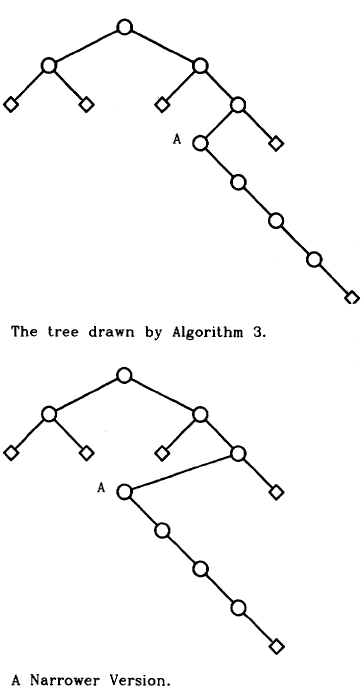
\includegraphics[scale = 0.75]{abbildungen/baum_theorem_uglification}
    \caption{Beispiel für das Theorem\cite[]{q1}}
    \label{pic:baum_theorem_uglification} 
\end{figure}

Bei der schmaleren Variante des Baumes auf Abbildung \ref{pic:baum_theorem_uglification} ist der Vater von Knoten A nicht zentriert
über beiden Kindern und verstößt somit gegen Aesthetic 3. Die weitere Variante verstößt gegen das physikalische Limit, da der Baum nicht
maximal schmal ist. Dies stellt hier einen Trade-off zwischen den beiden Anforderungen dar. Es ist somit möglich, dass maximal schmale Bäume der
Anforderungen Aesthetic 3 widersprechen können. 

Im Vergleich zu dem naiven Algorithmus von Wetherell und Shannon zeichnet der verbesserte Algorithmus die Bäume nicht mehr maximal links.
Dies sorgt dafür, dass die gezeichneten Bäume übersichtlicher wirken und ästhetisch ansprechender sind. Falls die Knoten einen Inhalt haben, dann
ist die Positionierung der Knoten auch von Relevanz, da das linke Kind kleiner und das rechte Kind größer als der Knoten ist. Beispielsweise
Suchbäume sind dadurch auch intuitiver zu verstehen, da die Größe des Inhalts von links nach rechts aufsteigend sortiert ist. 

Zudem ist der verbesserte Algorithmus nicht in der Lage beliebige Bäume zu zeichnen, sondern ausschließlich Binärbäume. Jedoch kann er durch
einige geeignete Erweiterungen so modifiziert werden, dass er auch in der Lage wäre beliebige Bäume zu zeichnen.
